\section{Android}

\subsection{Architecture}
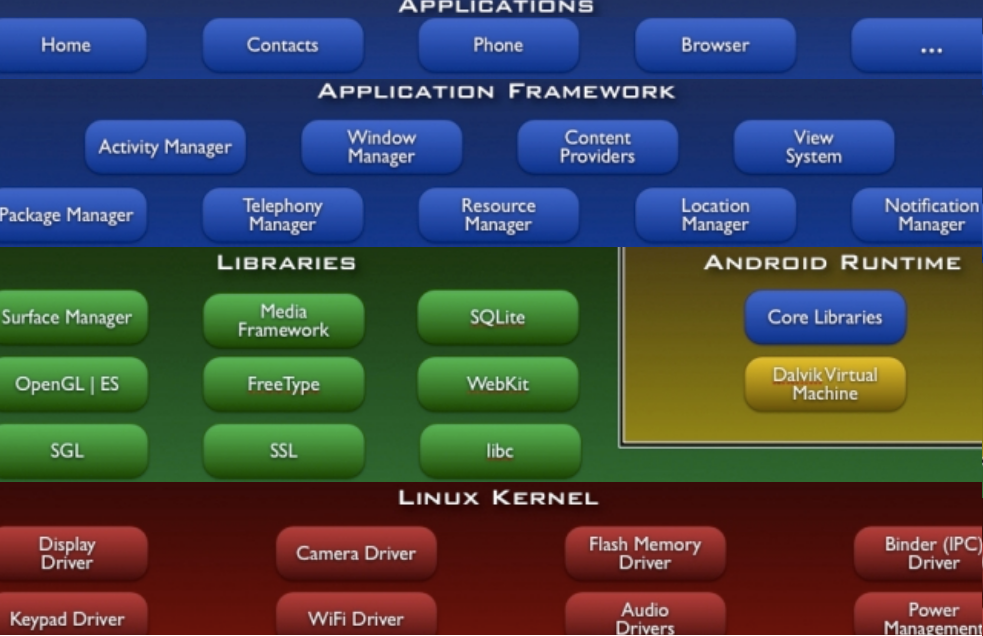
\includegraphics[width=0.15\textwidth]{android/architecture.png}
\textbf{Linux Kernel:} hardware abstraction layer (HAL), device drivers, memory
/ process management, networking

\textbf{Libraries:} C/C++ libraries. Interface through Java. Surface Manager.
2D and 3D Graphics. Media codecs, SQLite, Browser engine

\textbf{Android Runtime:}
Android runtime (ART) and its predecessor Dalvik are the managed runtime used
by apps and some system services.
Executes Dalvik Code (translated from Java bytecode).
Supports Ahead-of-time (AOT) compilation, garbage collections, profiling and
debugging.
Optimized for systems that are constrained in terms of memory and processor
speed.

\textbf{Application Framework:}
API interface, Activity manager (Manages the application life cycle).

\textbf{Applications:}
Built-in and user applications. Can replace built-in applications.

\subsubsection{Components}
App is built of Components that interacts. Goal: Easy to reuse and replace.
Components of other apps can be used (e.g. Gallery). Needs to be registered in
the AndroidManifest (<activity android:name=".ActivityB" />) (else exception).

\textbf{Activity}
User interface component typically corresponding to one screen. (Moving to next
screen means change of Activity).

\textbf{Service}
Runs in the background without user interface.
Example: music player, network download, etc
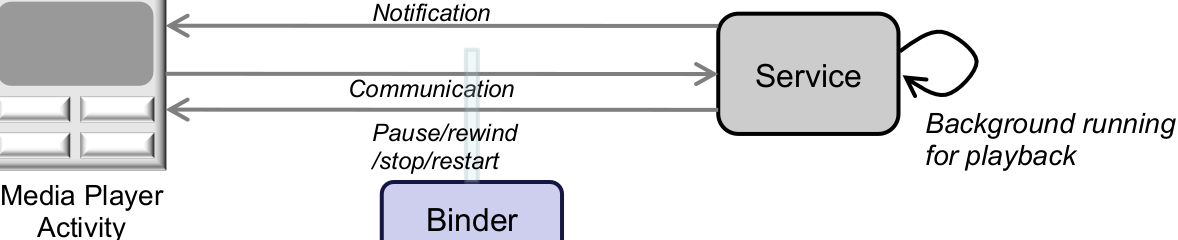
\includegraphics[width=0.15\textwidth]{android/service_example.png}

\textbf{Broadcast Receiver}
Component that receives and reacts to broadcast announcements (<- are Intents too).
Many broadcasts originate in system code (E.g., announcements that the time
zone has changed, that the battery is low. Incoming SMS)
Receiver are implemented by extending BroadcastReceiver.

\textbf{Content Provider}
recommended way to share data between Android applications (E.g. address book,
photo gallery). Represented by URI and MIME type.
Applications do not call content providers directly. They call ContentResolvers
instead as they typically do not reside in the same process.
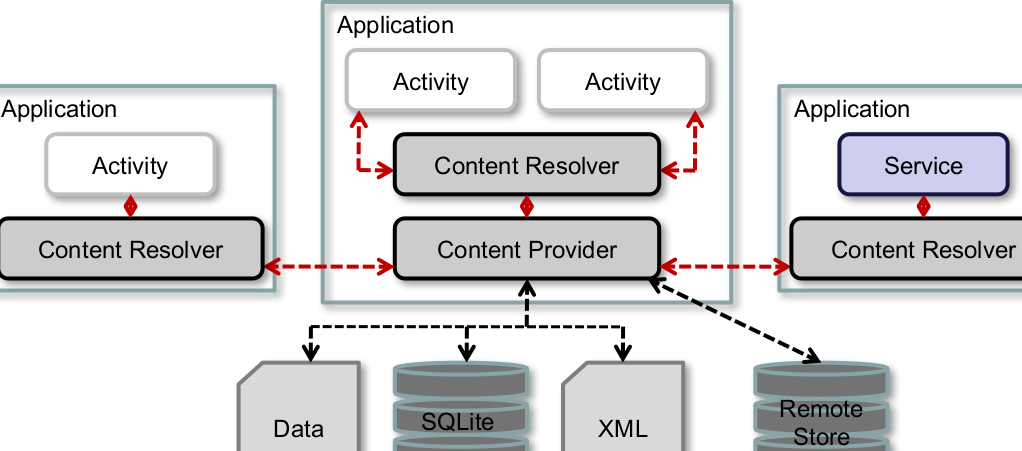
\includegraphics[width=0.15\textwidth]{android/content_provider.png}

\subsubsection{Transferring Program Control}
\textbf{Intents:} (Passive object, Set of Strings). Used for transfering
control or notify components (VIEW, CALL, PLAY, ...). Systems matches Intent
with most suitable.

\begin{lstlisting}
public void onClickSendBtn(final View btn){
  Intent intent = new Intent(this, Receiver.class);
  intent.putExtra("msg", "Hello World");
  startActivity(intent);
}
\end{lstlisting}

Android uses a requestId to \textbf{return results from a sub-activity}:
\begin{lstlisting}
startActivityForResult(new Intent(this, A.class), i1);
startActivityForResult(new Intent(this, B.class), i2);

// in sub-activity A or B
setResult(resultCode, intent); finish();

// back in main activity
@Override
protected void onActivityResult(int requestCode, int resultCode, Intent
data) {
  switch (requestCode) {
    case i1: // result from call with i1
    if (resultCode == RESULT_OK) { /* ... */ }
    break;
    case i2: // result from call with i2
    if (resultCode == RESULT_OK) { /* ... */ }
    break;
  }
}
\end{lstlisting}

\subsubsection{Activity Lifecycle}
State of an activity is managed by the system.

System may:
1) move another activity into the foreground.
2) ask the activity to finish.
3) even simply kill its process.

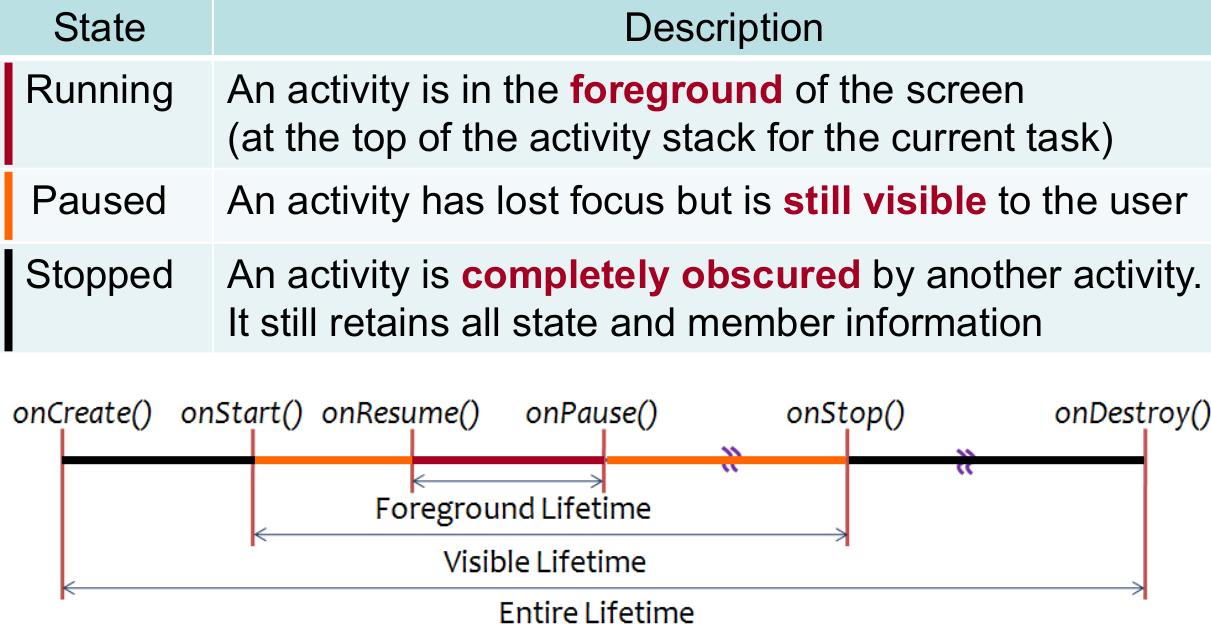
\includegraphics[width=0.15\textwidth]{android/activity_states.png}
System notifies an activity of a state transition by calling methods:
\textbf{onCreate:} first create or when activity was killed.
\textbf{onStart:} just before activity becomes visible.
\textbf{onRestart:} after activity has been stopped, to being started again.
\textbf{onResume:} before activity starts interacting with user (input goes to activity).
\textbf{onPause:} when about to resuming other activity (commit unsaved changes
here! stop animiations and CPU consumings)
\textbf{onStop:} when no longer visible to user (e.g. when destroyed or other activity resumed)
\textbf{onDestroy:} before destroy, but there is no guarantee.

\subsubsection{Configuration}
Advantages: Strings for localization, Images for different resolutions, Layouts for
different devices, ...

Seperated from code with resource files. Stored in \textbf{res} directory and
grouped by type: \textit{drawable}, \textit{layout}, \textit{values}. For
example \textit{res/values-de/strings.xml}
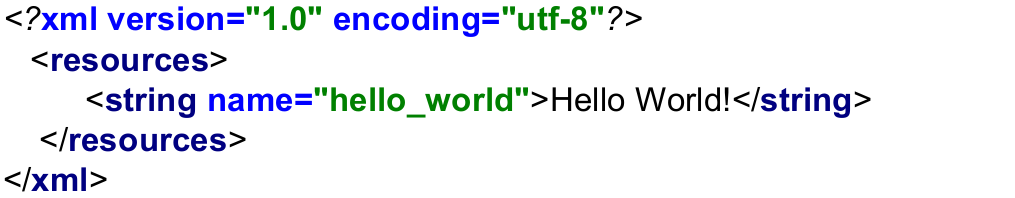
\includegraphics[width=0.15\textwidth]{android/example_resource.png}

Reference between resources with e.g. @string/hello_world.

Accessing resources in Java code with \textbf{wrapper class called R}, that
contains resource ids as static integers.

\begin{lstlisting}
// Load a custom layout for the current screen
setContentView(R.layout.main_screen);
// Set the text on a TextView object.
TextView view = (TextView)findViewByID(R.id.msg);
msgTextView.setText(R.string.hello_message);
// Set the title from a resource
this.getWindow().setTitle(Resources.getText(R.string.main_ title));
// Load a background for the current screen from a resource
this.getWindow().setBackgroundDrawableResource(R.drawable.my_background_image);
\end{lstlisting}

\subsubsection{AndroidManifest}
Properties of Application: Name / ID (package), Version of App, Technical User
(sharedUserId), Required SDK, Required Privileges, Components
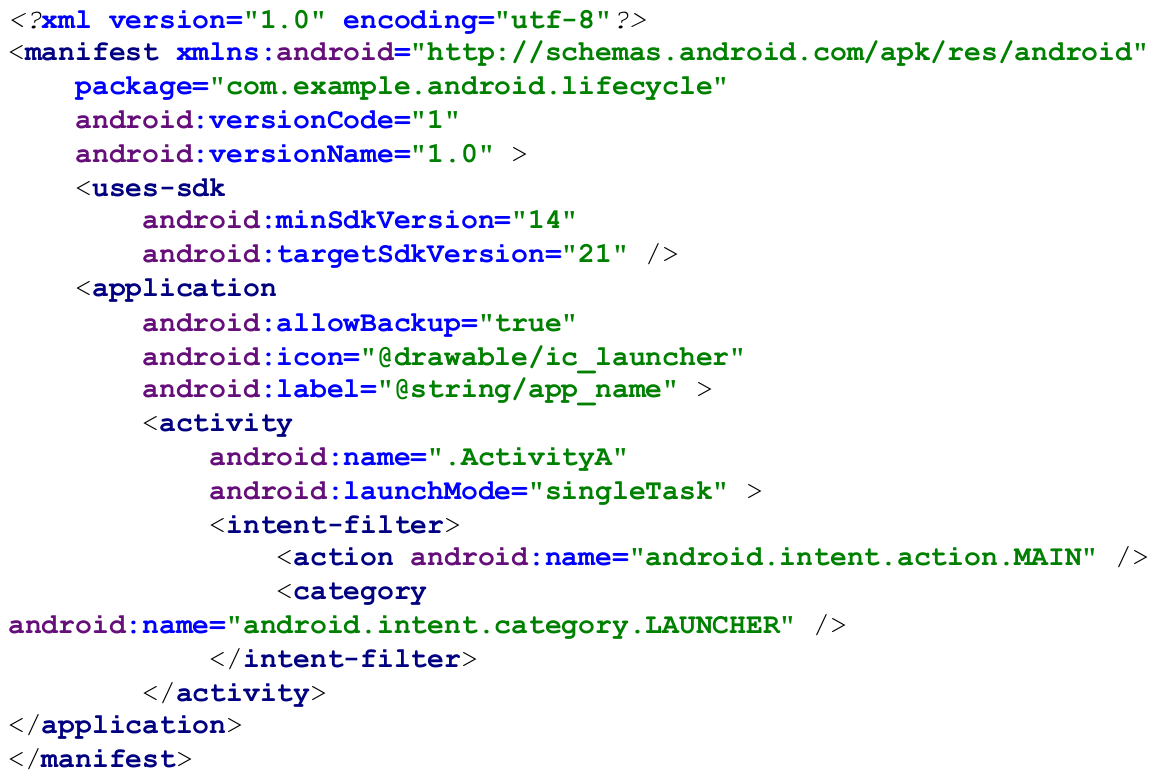
\includegraphics[width=0.15\textwidth]{android/manifest.png}
To be available from the launcher it must include an intent filter listening
for the MAIN action and the LAUNCHER category

\subsubsection{Application Lifecycle}


\newpage
\subsection{TODO SOME QUESTIONS OF BSKON EXAMS BECAUSE SAME TEACHER AND SAME CONTENT}
